\makeheading{Week 11}
\subsection{The \href{https://www.chehalemwines.com/}{Chehalem} Example}
\begin{itemize}
      \item Here we consider an example from \href{https://www.wiley.com/en-ca/Design+and+Analysis+of+Experiments C+10th+Edition-p-9781119492443}{Montgomery (2019)} in which a $ 2^{8-4} $ fractional factorial experiment
            was used in the production of wine to study the influence of a variety of factors on a particular vintage
            of Pinot Noir.
      \item In this experiment $K = 8$ factors were investigated each at two levels (the factors and their levels
            are shown in~\Cref{tab:wine1}) which, if a full factorial experiment was used, would have required 256
            conditions.
            \begin{table}[!htbp]
                  \centering
                  \caption{Factors and levels for the wine example.}\label{tab:wine1}
                  \begin{tabular}{lcc}
                        \toprule
                        Factor                       & Low ($ - $)           & High ($ + $)           \\
                        \midrule
                        Pinot Noir clone (A)         & Pommard               & Wädenswil              \\
                        Oak type (B)                 & Allier                & Tronçais               \\
                        Age of barrel (C)            & Old                   & New                    \\
                        Yeast/skin contact (D)       & Champagne             & Montrachet             \\
                        Stems (E)                    & None                  & All                    \\
                        Barrel toast (F)             & Light                 & Medium                 \\
                        Whole cluster (G)            & None                  & 10\%                   \\
                        Fermentation temperature (H) & Low (75$^\circ$F max) & High (92$^\circ$F max) \\
                        \bottomrule
                  \end{tabular}
            \end{table}
      \item To keep the experiment as small as possible a $ 2^{8-4}_{\text{IV}} $ fractional factorial experiment was performed that
            required only 16 conditions (i.e., 16 different wines).
      \item The response variable in this case is the rating of the wine as determined by 5 raters.
      \item Thus, 16 different wines were produced (based on the 16 unique combinations of these factors' levels)
            and $n = 5$ raters tasted and rated each of them (low scores are good, large scores are bad). The design
            matrix and a summary of the response is provided in~\Cref{tab:wine2}.
            \begin{table}[!htbp]
                  \centering
                  \caption{Design matrix and response summary for the $2^{8-4}$ fractional factorial wine experiment.}\label{tab:wine2}
                  \begin{tabular}{cccccccccc}
                        \toprule
                        Condition & A    & B    & C    & D    & $\text{E}=\text{BCD}$ & $\text{F}=\text{ACD}$ & $\text{G}=\text{ABC}$ & $\text{H}=\text{ABD}$ & $\text{Average Rating}=\bar{y}$ \\
                        \midrule
                        1         & $-1$ & $-1$ & $-1$ & $-1$ & $-1$                  & $-1$                  & $-1$                  & $-1$                  & $9.6$                           \\
                        2         & $+1$ & $-1$ & $-1$ & $-1$ & $-1$                  & $+1$                  & $+1$                  & $+1$                  & $10.8$                          \\
                        3         & $-1$ & $+1$ & $-1$ & $-1$ & $+1$                  & $-1$                  & $+1$                  & $+1$                  & $12.6$                          \\
                        4         & $+1$ & $+1$ & $-1$ & $-1$ & $+1$                  & $+1$                  & $-1$                  & $-1$                  & $9.2$                           \\
                        5         & $-1$ & $-1$ & $+1$ & $-1$ & $+1$                  & $+1$                  & $+1$                  & $-1$                  & $9.0$                           \\
                        6         & $+1$ & $-1$ & $+1$ & $-1$ & $+1$                  & $-1$                  & $-1$                  & $+1$                  & $15.0$                          \\
                        7         & $-1$ & $+1$ & $+1$ & $-1$ & $-1$                  & $+1$                  & $-1$                  & $+1$                  & $5.0$                           \\
                        8         & $+1$ & $+1$ & $+1$ & $-1$ & $-1$                  & $-1$                  & $+1$                  & $-1$                  & $15.2$                          \\
                        9         & $-1$ & $-1$ & $-1$ & $+1$ & $+1$                  & $+1$                  & $-1$                  & $+1$                  & $2.2$                           \\
                        10        & $+1$ & $-1$ & $-1$ & $+1$ & $+1$                  & $-1$                  & $+1$                  & $-1$                  & $7.0$                           \\
                        11        & $-1$ & $+1$ & $-1$ & $+1$ & $-1$                  & $+1$                  & $+1$                  & $-1$                  & $8.8$                           \\
                        12        & $+1$ & $+1$ & $-1$ & $+1$ & $-1$                  & $-1$                  & $-1$                  & $+1$                  & $2.8$                           \\
                        13        & $-1$ & $-1$ & $+1$ & $+1$ & $-1$                  & $-1$                  & $+1$                  & $+1$                  & $4.6$                           \\
                        14        & $+1$ & $-1$ & $+1$ & $+1$ & $-1$                  & $+1$                  & $-1$                  & $-1$                  & $2.4$                           \\
                        15        & $-1$ & $+1$ & $+1$ & $+1$ & $+1$                  & $-1$                  & $-1$                  & $-1$                  & $9.2$                           \\
                        16        & $+1$ & $+1$ & $+1$ & $+1$ & $+1$                  & $+1$                  & $+1$                  & $+1$                  & $12.6$                          \\
                        \bottomrule
                  \end{tabular}
            \end{table}
      \item Because the response variable in this setting is continuous, we use linear regression to analyze the data
            from this experiment.
      \item Because only $2^4=16$ conditions were used, we can only fit a model with 16 regression coefficients. In
            the context of a full $2^4$ factorial experiment, this would be the model with 4 main effects, 6 two-factor
            interactions, 4 three-factor interactions and 1 four-factor interaction:
            \verbatiminput{verbatim/wineOUT1.txt}
      \item But this output does not involve the factors E, F, G or H –-- it only directly references factors A, B, C
            and D.
      \item This is because of confounding.
            \begin{itemize}
                  \item The BCD interaction estimate also corresponds to the main effect of E.
                  \item The ACD interaction estimate also corresponds to the main effect of F.
                  \item The ABC interaction estimate also corresponds to the main effect of G.
                  \item The ABD interaction estimate also corresponds to the main effect of H.
            \end{itemize}
      \item[*] While we cannot technically separate these effects, we assume that the three-factor interactions are
            negligible, and hence any significant effect observed is due to the aliased main effect.
      \item The same model summary from above is shown in below, but this time with factors E, F, G and H
            referenced instead of the three-factor interactions:
            \verbatiminput{verbatim/wineOUT2.txt}
            \begin{itemize}[*]
                  \item All main effects are significant except for factor H (fermentation temperature).
                  \item Also, the AC, AD, and AH interactions are significant. However, factors D, E, F, G, are \underline{most}
                        influential, so it's \underline{more likely} that the significance of these two-factor interactions is driven by aliased
                        interactions involving D, E, F, G.
                        \[ \text{AC}=\text{DF},\qquad\text{AD}=\text{EG},\qquad\text{AH}=\text{FG} \]
                  \item We will therefore speculate that it's the DF, EG, and FG interactions that are important.
            \end{itemize}
      \item \Cref{fig:wineME} depicts the main effect plots for all eight factors.
            \begin{figure}[!htbp]
                  \centering
                  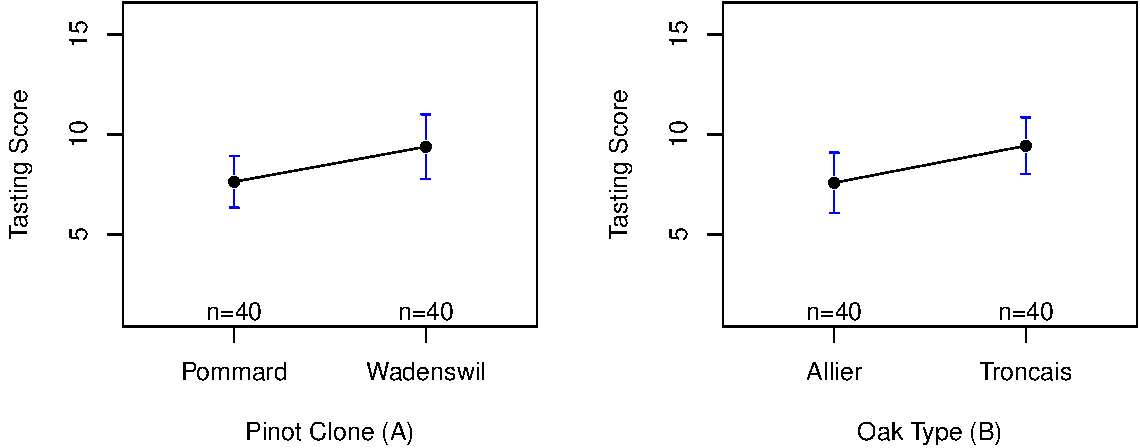
\includegraphics[width=.48\textwidth]{wineME1.pdf}\hfill
                  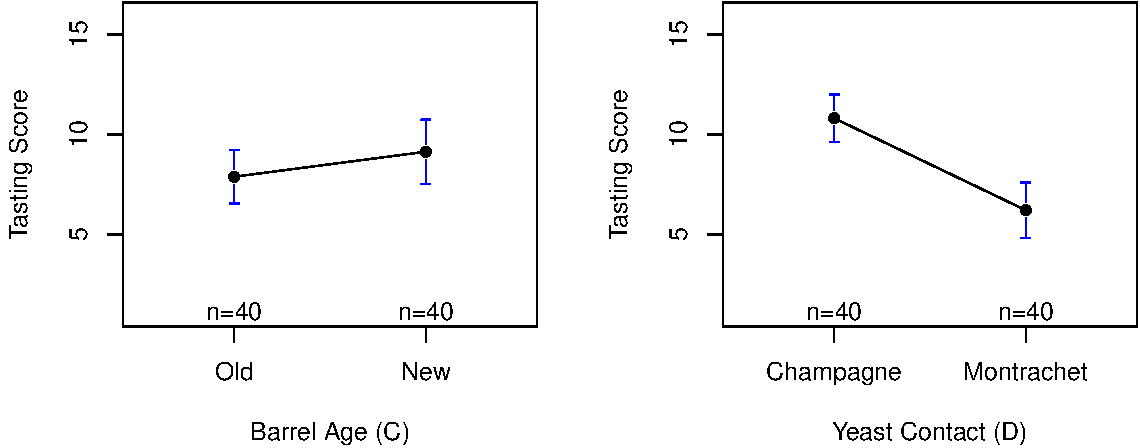
\includegraphics[width=.48\textwidth]{wineME2.pdf}
                  \\[\smallskipamount]
                  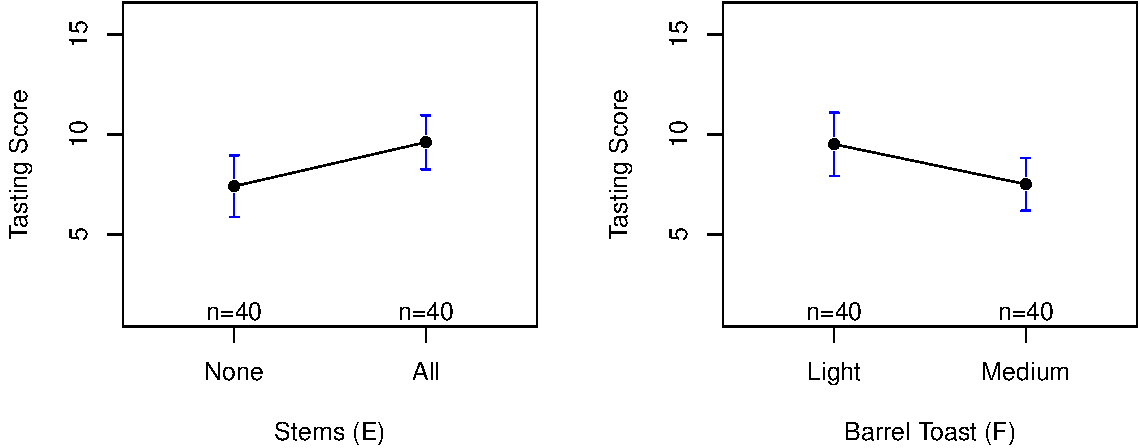
\includegraphics[width=.48\textwidth]{wineME3.pdf}\hfill
                  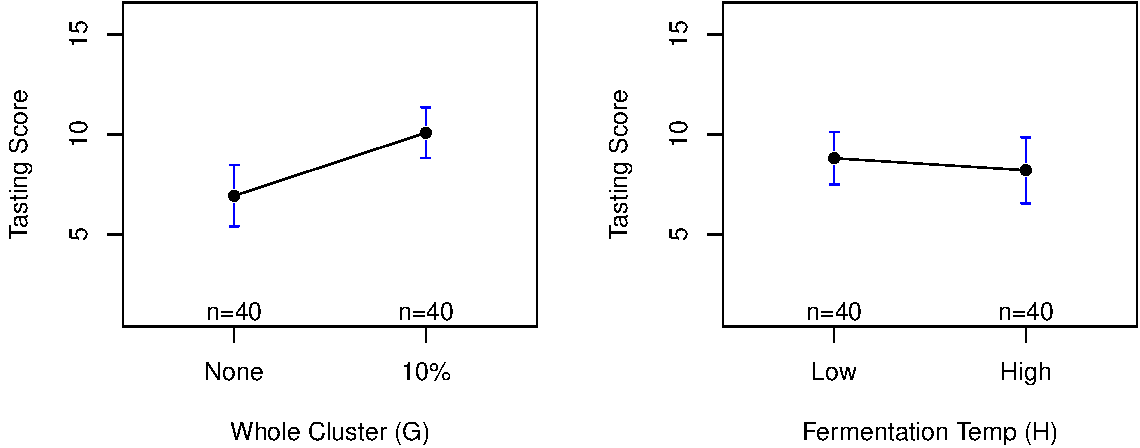
\includegraphics[width=.48\textwidth]{wineME4.pdf}
                  \caption{Main effect plots for the wine example.}\label{fig:wineME}
            \end{figure}
      \item \Cref{fig:wineIE} depicts the interaction effect plots for the three significant interactions.
            \begin{figure}[!htbp]
                  \centering
                  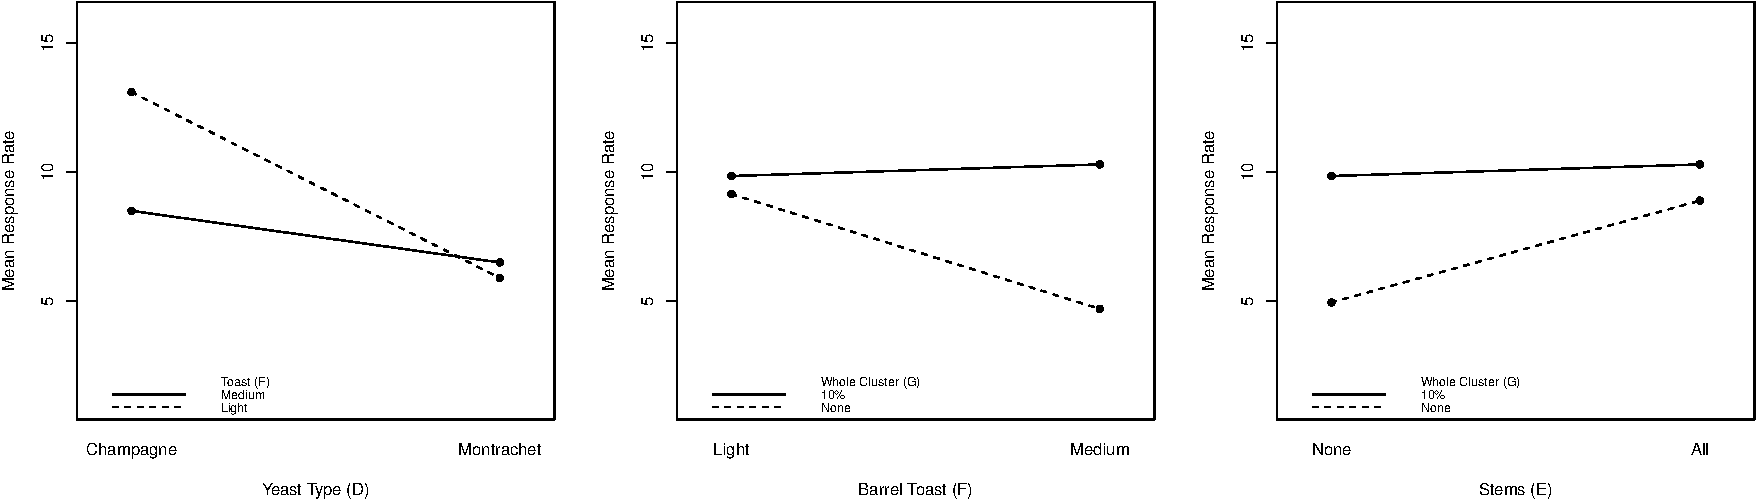
\includegraphics[width=\textwidth]{wineIE.pdf}
                  \caption{Interaction effect plots for the wine example.}\label{fig:wineIE}
            \end{figure}
            \begin{itemize}
                  \item If yeast type is Montrachet, then the effect of Barrel toast is minimal.
                  \item The effect of whole clusters is minimal if Barrel toast is light.
                  \item Effect of the whole cluster is minimal when all stems are used.
            \end{itemize}
\end{itemize}
\chapter{RESPONSE SURFACE METHODOLOGY}
\begin{itemize}
      \item[*] Effective experimentation is sequential
            \begin{itemize}
                  \item Information gained in one experiment can help to inform future experiments.
                  \item This is the philosophy of \textbf{response surface methodology}.
            \end{itemize}
      \item We have seen that the primary purpose of screening experiments is to identify which among numerous
            factors are the ones that significantly influence the response variable.
            \begin{itemize}[$\hookrightarrow$]
                  \item \underline{Phase 1}: Factor screening with two-level designs.
            \end{itemize}
      \item[*] Now we discuss how screening experiments may be followed-up by further experiments whose primary
            purpose is response optimization.
            \begin{itemize}[$\hookrightarrow$]
                  \item We use the method of \textbf{steepest ascent/descent} (phase 2) and \textbf{response surface designs} (phase 3) to locate
                        optimal settings of the factors that were identified as significant in the screening phase.
                        \begin{itemize}
                              \item Phase 4: Confirmation.
                        \end{itemize}
            \end{itemize}
\end{itemize}
\section{Overview of Response Optimization}
\subsection*{Coded Factors}
\begin{itemize}
      \item Here we consider $ K^\prime\le K $ design factors which are a subset of the $K$ factors investigated during the
            screening phase.
      \item The set of possible values these factors can take on is referred to as the \textbf{region of operability}.
            \begin{itemize}
                  \item[*] It is this region that we explore and in which we run our experiments to determine the \emph{optimal}
                        operating condition.
                        \begin{Example}{}{}
                              If the design factor is discount amount, then the region of operability is $ [0,100] $.
                        \end{Example}
            \end{itemize}
      \item Although this region specifies acceptable factor values in their natural units (such as dollars, minutes,
            percent, etc.), we typically work on a transformed scale.
      \item Just like in the regression models used in the experiments, we represent each factor by a coded variable
            $x$ that takes on the values $-1$ and $+1$ when the factor is at its \emph{low} and \emph{high} levels.
            \begin{itemize}
                  \item[*] When the factor is categorical this coding is arbitrary.
                  \item When the factor is numeric the coding arises through the following transformation:
                        \[ x=\frac{U-(U_{\symbfsfup{H}}+U_{\symbfsfup{L}})/2}{(U_{\symbfsfup{H}}-U_{\symbfsfup{L}})/2}  \]
                        \begin{itemize}
                              \item $ U $ is \underline{any} value of the factor in natural units.
                                    \begin{itemize}
                                          \item $ U_{\symbfsfup{H}} $ and $ U_{\symbfsfup{L}} $ are ``high'' and ``low'' levels of the factor recorded in natural units.
                                    \end{itemize}
                              \item $ x $ is the transformed version of $ U $ in coded units.
                                    \begin{itemize}
                                          \item If $ U=U_{\symbfsfup{H}} $, then $ x=+1 $, and if $ U=U_{\symbfsfup{L}} $, then $ x=-1 $.
                                    \end{itemize}
                        \end{itemize}
                        \begin{Example}{}{}
                              Assume we're experimenting with discount amount where $ U_{\symbfsfup{L}}=20\% $ and $ U_{\symbfsfup{H}}=50\% $.
                              Then $ x=(U-35)/15 $ may be used to convert from natural units to coded units.
                              \begin{itemize}[leftmargin=5mm]
                                    \item If $ U=50 $, then $ x=+1 $.
                                    \item If $ U=20 $, then $ x=-1 $.
                                    \item If $ U=40 $, then $ x=1/3 $.
                                    \item If $ U=60 $, then $ x=5/3 $.
                              \end{itemize}
                        \end{Example}
                  \item This equation may also be inverted allowing for conversion from the coded units back to the
                        natural units as follows:
                        \[ U=x\times \frac{U_{\symbfsfup{H}}-U_{\symbfsfup{L}}}{2}+\frac{U_{\symbfsfup{H}}+U_{\symbfsfup{L}}}{2}  \]
                        \begin{itemize}
                              \item Translating from coded to natural units is especially useful when translating the location of
                                    the optimum from coded units to natural units.
                                    \begin{Example}{}{}
                                          Optimal $ x=1.45\rightarrow U=1.45(15)+35=56.75\% $.
                                    \end{Example}
                        \end{itemize}
            \end{itemize}
      \item Adopting this notation, the objective of response optimization may be stated as determining the value
            of $ \Vector{x}=(x_1,x_2,\ldots,x_{K^\prime})^\top $ (and hence $ \Vector{U}=(U_1,U_2,\ldots,U_{K^\prime})^\top $)
            at which we expect the response to be optimized.
\end{itemize}
\subsection*{The Models}
\begin{itemize}
      \item The goal of response optimization may be achieved via \textbf{response surface experimentation} where
            one seeks to characterize the relationship between the expected response $ \E{Y} $ and the $ K^\prime $ design factors.
      \item In the case of a continuous response, we may write this relationship generally as:
            \[ \E{Y}=f(x_1,x_2,\ldots,x_{K^\prime}) \]
            and in the case of a binary response:
            \[ \log*{\frac{\E{Y}}{1-\E{Y}}}=f(x_1,x_2,\ldots,x_{K^\prime}) \]
      \item In both cases, the function $ f(x_1,x_2,\ldots,x_{K^\prime}) $ represents the \emph{true} but \emph{unknown} \textbf{response surface}.
            \begin{itemize}
                  \item If we knew $ f(\:\cdot\:) $, we could easily find the values of $ x_1,\ldots,x_{K^\prime} $ that optimize it.
            \end{itemize}
      \item Because $ f(\:\cdot\:) $ is unknown, we must fit models that approximate this surface. As usual, we use linear
            and logistic regression.
      \item Although many models may be used to approximate the response surface we exploit Taylor's
            Theorem and use \emph{low-order polynomials}:
            \begin{itemize}
                  \item First-order model:
                        \[ \eta=\beta_0+\beta_1x_1+\beta_2x_2+\cdots+\beta_{K^\prime}x_{K^\prime} \]
                        \begin{itemize}[$\hookrightarrow$]
                              \item Main effects only.
                        \end{itemize}
                  \item First-order + Interaction model:
                        \[ \eta=\beta_0+\sum_{j=1}^{K^\prime} \beta_j x_j+\sum_{j<\ell}\beta_{j\ell}x_j x_\ell  \]
                        \begin{itemize}[$\hookrightarrow$]
                              \item Main effect + two-factor interactions.
                        \end{itemize}
                  \item Second-order model:
                        \[ \eta=\beta_0+\sum_{j=1}^{K^\prime}\beta_j x_j+\sum_{j<\ell}\beta_{j\ell}x_j x_\ell+\sum_{j=1}^{K^\prime}\beta_{jj}x_j^2  \]
                        \begin{itemize}[$\hookrightarrow$]
                              \item Quadratic effects in addition to main effects and two-factor interactions.
                        \end{itemize}
            \end{itemize}
      \item Examples of such response surfaces (for $ K^\prime=2 $) are visualized in~\Cref{fig:respsurfaces}:
            \begin{figure}[!htbp]
                  \centering
                  \begin{subfigure}{0.5\textwidth}
                        \centering
                        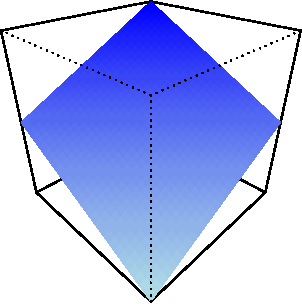
\includegraphics[width=.48\linewidth]{FO1.pdf}
                        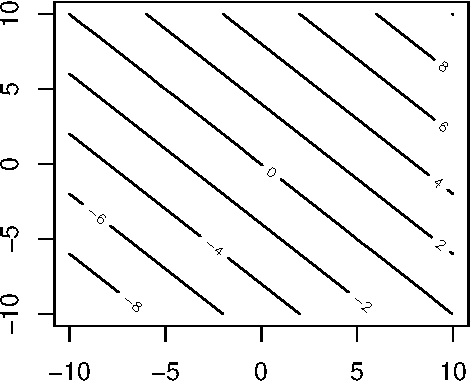
\includegraphics[width=.48\linewidth]{FO2.pdf}
                        \caption{$\eta=\beta_0+\beta_1x_1+\beta_2x_2$ (Plane)}\label{fig:plane}
                  \end{subfigure}
                  \begin{subfigure}{0.5\textwidth}
                        \centering
                        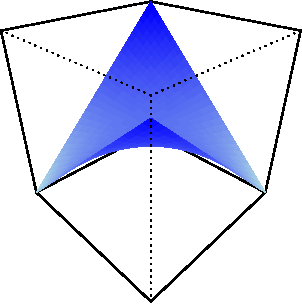
\includegraphics[width=.48\linewidth]{FOI1.pdf}
                        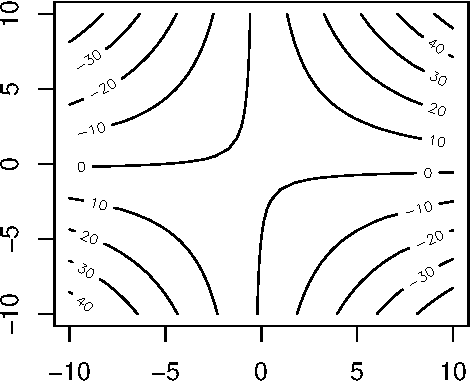
\includegraphics[width=.48\linewidth]{FOI2.pdf}
                        \caption{$\eta=\beta_0+\beta_1x_1+\beta_2x_2+\beta_{12}x_1x_2$ (Twisted Plane)}\label{fig:twplane}
                  \end{subfigure}
                  \begin{subfigure}{0.5\textwidth}
                        \centering
                        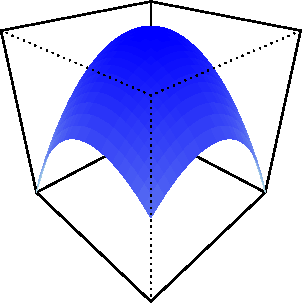
\includegraphics[width=.48\linewidth]{SO1.pdf}
                        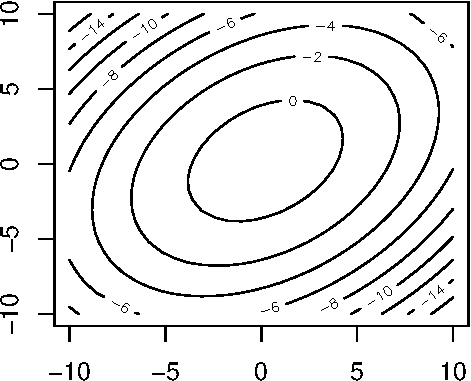
\includegraphics[width=.48\linewidth]{SO2.pdf}
                        \caption{$\eta=\beta_0+\beta_1x_1+\beta_2x_2+\beta_{12}x_1x_2+\beta_{11}x_1^2+\beta_{22}x_2^2$}\label{fig:secondorder}
                  \end{subfigure}
                  \caption{Example 3D surface and 2D contour plots of first-order (\Cref{fig:plane}), first-order-plus-interaction (\Cref{fig:twplane})
                        and second-order (\Cref{fig:secondorder}) response surfaces.}\label{fig:respsurfaces}
            \end{figure}
      \item[*] We must acknowledge that the approximation of $ f(x_1,x_2,\ldots,x_{K^\prime}) $ by $ \eta $ (regardless of whether $ \eta $ is
            first-order or second-order) is likely to be poor when considered across the entire $x$-space.
            \begin{itemize}[$\rightarrow$]
                  \item However, in the small localized region of an experiment, such low-order polynomials should well-
                        approximate $ f(\:\cdot\:) $.
            \end{itemize}
      \item[$\rightarrow$] Which model is appropriate is dictated by the goal of the experiment.
            \begin{itemize}
                  \item In the context of factor screening we saw that first-order and first-order-plus-interaction models
                        suited our needs.
                  \item But in order to identify maxima/minima we require the second-order model as it is capable of
                        modelling concavity/convexity.
                  \item Therefore, second-order models are used for response surface optimization.
            \end{itemize}
\end{itemize}
\section{Method of Steepest Ascent/Descent}
\begin{itemize}
      \item We use the method of steepest of ascent/descent to determine \emph{roughly} where in the $x$-space the optimum
            lies.
            \begin{itemize}
                  \item Hence, this tells us where a response surface design and a second-order model would be most
                        useful.
                  \item[*] We want to find the ``vicinity'' of the optimum.
            \end{itemize}
      \item[*] The method is gradient-based and designed to identify the direction that when traversed moves you
            toward the optimum as quickly as possible.
\end{itemize}
\subsection{The Path of Steepest Ascent/Descent}
\begin{itemize}
      \item We use a $ 2^{K^\prime} $ (or $ 2^{K^\prime-p} $) factorial experiment to estimate a \emph{first-order response surface}:
            \[ \hat{\eta}=\hat{\beta}_0+\hat{\beta}_1x_1+\hat{\beta}_2x_2+\cdots+\hat{\beta}_{K^\prime}x_{K^\prime} \]
      \item The gradient of this surface is then calculated:
            \[ \Vector{g}=\nabla \hat{\eta}=\biggl(\pdv{\hat{\eta}}{x_1},\pdv{\hat{\eta}}{x_2},\ldots,\pdv{\hat{\eta}}{x_{K^\prime}}\biggr)^{\!\top} \]
            \begin{itemize}
                  \item This gradient defines the \textbf{path of steepest ascent/descent} (i.e., the direction of steepest increase/decrease on the fitted surface).
                  \item If maximizing the response is of interest, then we should ascend the surface by moving in the
                        direction of $ +\Vector{g} $:
                        \begin{equation}
                              \Vector{x}^\prime=\Vector{x}+\lambda \Vector{g}\label{eq:maxgr}\tag*{(1)}
                        \end{equation}
                  \item If minimizing the response is of interest, then we should descend the surface by moving in the
                        direction of $ -\Vector{g} $:
                        \begin{equation}
                              \Vector{x}^\prime=\Vector{x}-\lambda \Vector{g}\label{eq:mingr}\tag*{(2)}
                        \end{equation}
                  \item With a fixed step size $ \lambda $ we move from $ \Vector{x} $ to $ \Vector{x}^\prime $.
                  \item We typically define the step size as:
                        \[ \lambda=\frac{\Delta x_j}{\abs{\hat{\beta}_j}}  \]
                        \begin{itemize}
                              \item Pick factor $ j $, the one you know the most about, or the one that is hardest to manipulate.
                              \item $ \Delta x_j $ is the step size of factor $ j $ in coded units.
                              \item $ \hat{\beta}_j $ is the estimated coefficient corresponding to factor $ j $ in the estimated first-order response model.
                        \end{itemize}
            \end{itemize}
\end{itemize}
\begin{framed}
      \textbf{Steepest Ascent/Descent Algorithm}
      \begin{enumerate}[1.]
            \item The first condition along the path of steepest ascent/descent is at the origin of the $x$-space
                  $ \Vector{x}_0=(0,0)^\top $ (i.e., the centre of the $ 2^{K^\prime} $ factorial design that was used to fit $ \hat{\eta} $).
                  Data is collected and the metric of interest is calculated.
            \item Then the step size $ \lambda $ is determined.
            \item The location of the next condition is determined by formula~\ref{eq:maxgr} in the case of maximization and~\ref{eq:mingr} in the case of minimization. Data is collected and the metric of interest is calculated.
            \item Repeat Step 3 until incremental improvements in the MOI cease.
            \item Return to the location of the best MOI value and \emph{test for curvature}.
                  \begin{itemize}[$\rightarrow$]
                        \item If the test for curvature suggests that you are not yet in the vicinity of the optimum, fit a
                              new first-order model and repeat Steps 1 to 4.
                        \item If the test for curvature suggests that you are in the vicinity of the optimum, use a response
                              surface design to fit a full second-order model and hence precisely identify the coordinates of
                              the optimum.
                  \end{itemize}
      \end{enumerate}
\end{framed}
\subsection{Checking for Curvature}
\begin{itemize}
      \item A test for quadratic curvature is an important component of the method of steepest ascent/descent.
            \begin{itemize}
                  \item[*] The presence of quadratic curvature signifies that you are in the vicinity of the optimum.
            \end{itemize}
      \item Such a test is possible when a $ 2^{K^\prime} $ factorial experiment is augmented with a \textbf{centre point} condition.
            \begin{itemize}
                  \item The centre point condition is defined (in coded units) as $ x_1=x_2=\cdots=x_{K^\prime}=0 $.
                  \item Located at the centre of the cuboidal region defined by the $ 2^{K^\prime} $ factorial conditions.
            \end{itemize}
      \item[*] The data arising from a $ 2^{K^\prime} $ factorial design is insufficient to estimate a second-order linear predictor.
            \begin{itemize}
                  \item[*] We are able to estimate the main effects and the two-factor interaction effects, but \emph{not} the quadratic effects.
            \end{itemize}
      \item With the addition of the centre point condition, one \emph{additional} effect may be estimated: the \textbf{pure quadratic effect}.
            \[ \beta_{\symbfsfup{PQ}}=\sum_{j=1}^{K^\prime} \beta_{jj} \]
      \item A test of $ \HN $: $ \beta_{\symbfsfup{PQ}}=0 $ is a test of \emph{overall curvature}.
\end{itemize}
\begin{Example}{$ K^\prime=2 $}{}
      \begin{itemize}
            \item When $ K^\prime=2 $, the second-order linear predictor is:
                  \[ \eta=\beta_0+\beta_1x_1+\beta_2x_2+\beta_{12}x_1x_2+\beta_{11}x_1^2+\beta_{22}x_2^2 \]
            \item In a $ 2^2 $ factorial design plus a centre point, we have the following five unique experimental conditions:
                  $ (x_1,x_2)\in\Set[\big]{(−1, −1), (+1, −1), (−1, +1), (+1, +1), (0, 0)} $ which respectively give rise to
                  five unique variants of the linear predictor, which we define as:
                  \[ \eta_{\symbfsfup{LL}}=\beta_0-\beta_1-\beta_2+\beta_{12}+\beta_{11}+\beta_{22} \]
                  \[ \eta_{\symbfsfup{HL}}=\beta_0+\beta_1-\beta_2-\beta_{12}+\beta_{11}+\beta_{22} \]
                  \[ \eta_{\symbfsfup{LH}}=\beta_0-\beta_1+\beta_2-\beta_{12}+\beta_{11}+\beta_{22} \]
                  \[ \eta_{\symbfsfup{HH}}=\beta_0+\beta_1+\beta_2+\beta_{12}+\beta_{11}+\beta_{22} \]
                  \[ \eta_{\symbfsfup{C}}=\beta_0 \]
            \item[*] With only these five conditions, we cannot separately estimate $ \beta_{11} $ and $ \beta_{22} $,
                  but we \emph{can} estimate $ \beta_{\symbfsfup{PQ}}=\beta_{11}+\beta_{22} $.
            \item Notice that:
                  \[ \beta_{\symbfsfup{PQ}}=\frac{\eta_{\symbfsfup{LL}}+\eta_{\symbfsfup{HL}}+\eta_{\symbfsfup{LH}}+\eta_{\symbfsfup{HH}}}{4}-\eta_{\symbfsfup{C}}  \]
            \item The estimate is therefore:
                  \[ \hat{\beta}_{\symbfsfup{PQ}}=\frac{\hat{\eta}_{\symbfsfup{LL}}+\hat{\eta}_{\symbfsfup{HL}}+\hat{\eta}_{\symbfsfup{LH}}+\hat{\eta}_{\symbfsfup{HH}}}{4}-\hat{\eta}_{\symbfsfup{C}}  \]
                  \begin{itemize}[*]
                        \item If this difference, and hence $ \hat{\beta}_{\symbfsfup{PQ}} $, is small then it suggests that the response values
                              observed in the factorial conditions are similar to those observed in the centre point condition and hence that there isn't
                              significant curvature in the response surface.
                        \item If $ \hat{\beta}_{\symbfsfup{PQ}} $ is very different from zero, it suggests that there is significant quadratic curvature.
                  \end{itemize}
            \item We formally test $ \HN $: $ \hat{\beta}_{\symbfsfup{PQ}} $ using $t$-tests (or $Z$-tests) in a linear (or logistic) regression model
                  that has linear predictor:
                  \[ \eta=\beta_0+\beta_1x_1+\beta_2x_2+\beta_{12}x_1x_2+\beta_{\symbfsfup{PQ}}x_{\symbfsfup{PQ}} \]
                  where
                  \[ x_{\symbfsfup{PQ}}=\begin{cases}
                              1 & (x_1,x_2)\in\Set[\big]{(-1,-1),(+1,-1),(-1,+1),(+1,+1)} \\
                              0 & (x_1,x_2)=(0,0)
                        \end{cases} \]
                  which indicates whether a response observation came from a factorial condition or the centre point condition.
            \item If $ \beta_{\symbfsfup{PQ}} $ is significantly different from 0 then it suggests that \emph{both} $ \beta_{11} $ and $ \beta_{22} $
                  are significantly non-zero, and therefore that there is significant quadratic curve.
      \end{itemize}
\end{Example}
\begin{itemize}
      \item For general $ K^\prime $, we conduct a $ 2^{K^\prime} $ factorial experiment with a centre point and then test for curvature
            using a regression model with linear predictor:
            \[ \eta=\beta_0+\sum_{j=1}^{K^\prime} \beta_j x_j+\sum_{j<\ell}\beta_{j\ell}x_j x_\ell+\beta_{\symbfsfup{PQ}}x_{\symbfsfup{PQ}} \]
            where now
            \[ \beta_{\symbfsfup{PQ}}=\sum_{j=1}^{K^\prime} \beta_{jj} \]
            and $ x_{\symbfsfup{PQ}} $ is again a binary indicator indicating whether a response value was observed in a factorial
            condition or the centre point condition.
      \item[*] No matter the value of $ K^\prime $, the pure quadratic effect is always represented by a single term in the model.
            \begin{itemize}
                  \item As such, the test for curvature is always a test of $ \HN $: $ \beta_{\symbfsfup{PQ}}=0 $ and is carried out with ordinary
                        $t$-tests in a linear regression and $Z$-tests in a logistic regression.
            \end{itemize}
      \item The intuitive estimate for $ \beta_{\symbfsfup{PQ}} $ in the $ K^\prime=2 $ case also generalizes:
            \[ \hat{\beta}_{\symbfsfup{PQ}}=\hat{\bar{\eta}}_{\symbfsfup{F}}-\hat{\eta}_{\symbfsfup{C}} \]
            where
            \begin{itemize}[$\rightarrow$]
                  \item $ \hat{\bar{\eta}}_{\symbfsfup{F}} $ is the average if the estimated linear predictor values in the factorial conditions.
                  \item $ \hat{\eta}_{\symbfsfup{C}} $ is the estimated linear predictor value at the centre point.
            \end{itemize}
      \item \textbf{IMPORTANT}: This test assumes that all the $ \beta_{jj} $'s, $ j=1,2,\ldots,K^\prime $, have the same sign.
            \begin{itemize}
                  \item If they didn't, then it's possible that significantly large $ \beta_{jj} $'s could cancel each other out, making
                        $ \beta_{\symbfsfup{PQ}}=\sum_{j=1}^{K^\prime} \beta_{jj} $ close to zero.
                        \begin{itemize}[$\hookrightarrow$]
                              \item We are misled into thinking that we are not in the vicinity of the quadratic curvature, even when we are.
                        \end{itemize}
                  \item[*] This assumption is fine as long as the experiment is not conducted near a saddle point on the
                        response surface.
                        \begin{itemize}[$\hookrightarrow$]
                              \item This problem can only be identified by separately estimating each of the quadratic effects.
                        \end{itemize}
            \end{itemize}
\end{itemize}
\subsection{The Netflix Example}
\begin{itemize}
      \item Here we illustrate the \emph{method of steepest descent} using a modified version of the hypothetical Netflix
            experiment from your final project.
      \item We focus on the Preview Length factor (defined analogously as in your project) and a Preview Size
            factor (which corresponds to the size of the enlarged window a preview is played in).
      \item We begin with a $2^2$ factorial experiment with a centre point condition. The factor levels in coded and
            natural units are shown in~\Cref{tab:netflixtab1}.
            \begin{table}[!htbp]
                  \centering
                  \caption{Average browsing time by condition in the $2^2 + \symbfsfup{CP}$ Netflix experiment.}\label{tab:netflixtab1}
                  \begin{tabular}{cccccc}
                        \toprule Condition & Preview Length & $x_{1}$ & Preview Size & $x_{2}$ & Average Browsing Time \\
                        \midrule 1         & 90 seconds     & $-1$    & $0.2$        & $-1$    & $22.16$ minutes       \\
                        2                  & 120 seconds    & $+1$    & $0.2$        & $-1$    & $22.20$ minutes       \\
                        3                  & 90 seconds     & $-1$    & $0.5$        & $+1$    & $20.22$ minutes       \\
                        4                  & 120 seconds    & $+1$    & $0.5$        & $+1$    & $21.98$ minutes       \\
                        5                  & 105 seconds    & 0       & $0.35$       & 0       & $22.05$ minutes       \\
                        \bottomrule
                  \end{tabular}
            \end{table}
      \item Prior to embarking down the path of steepest descent, a curvature test was performed to determine
            whether this experimental region was already in the vicinity of the optimum.
      \item The linear regression model with linear predictor:
            \[ \eta=\beta_0+\beta_1x_1+\beta_2x_2+\beta_{12}x_1x_2+\beta_{\symbfsfup{PQ}}x_{\symbfsfup{PQ}} \]
            was fit. The resulting output is shown below:
            \verbatiminput{verbatim/netflixOUT1.txt}
      \item To begin the method of steepest descent procedure, we use the aforementioned data to fit the first
            order regression model with linear predictor:
            \[ \hat{\eta}=\hat{\beta}_0+\hat{\beta}_1x_1+\hat{\beta}_2x_2 \]
            The model summary is shown below:
            \verbatiminput{verbatim/netflixOUT2.txt}
      \item \Cref{fig:nf1} depicts the contours of the estimated first-order response surface.
            \begin{figure}[!htbp]
                  \centering
                  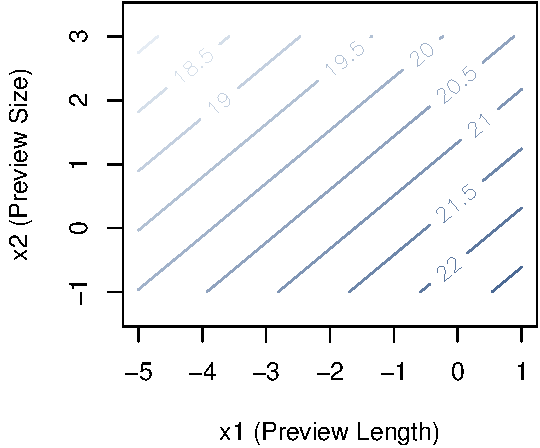
\includegraphics[width=0.5\textwidth]{nf1.pdf}
                  \caption{Contour plot for the estimated first-order response surface for the Netflix experiment.}\label{fig:nf1}
            \end{figure}
      \item We calculate the gradient:
            \[ \Vector{g}=(\hat{\beta}_1,\hat{\beta}_2)^\top=\biggl(\pdv{\hat{\eta}}{x_1},\pdv{\hat{\eta}}{x_2}\biggr)^{\!\top}=(0.44828,-0.53894)^\top \]
      \item[*] This path of steepest descent is depicted by the dashed black line in~\Cref{fig:nf2}. The red dots signify
            the experimental conditions conducted along this path, beginning from the centre point $ (x_1,x_2)=(0,0) $.
            \begin{figure}[!htbp]
                  \centering
                  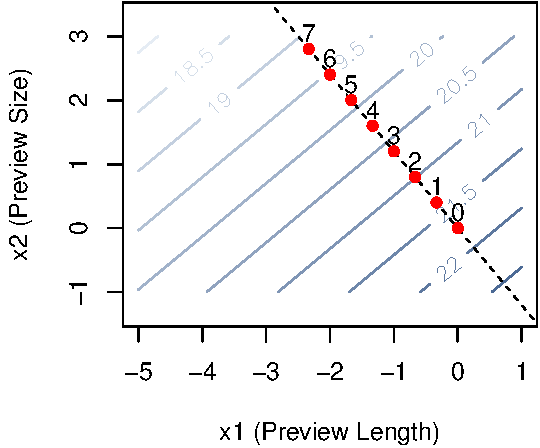
\includegraphics[width=0.5\textwidth]{nf2.pdf}
                  \caption{Contour plot for the path of steepest descent for the Netflix experiment.}\label{fig:nf2}
            \end{figure}
      \item The locations in coded and natural units for each of these conditions are provided in~\Cref{tab:netflixtab2}.
            \begin{table}[!htbp]
                  \centering
                  \caption{Average browsing time along the path of steepest descent.}\label{tab:netflixtab2}
                  \begin{tabular}{cccccc}
                        \toprule Step & Preview Length & $x_{1}$  & Preview Size & $x_{2}$     & Average Browsing Time \\
                        \midrule 0    & 105 seconds    & 0        & $0.3500000$  & 0           & $22.00$ minutes       \\
                        1             & 100 seconds    & $-1 / 3$ & $0.4101118$  & $0.4007454$ & $21.67$ minutes       \\
                        2             & 95 seconds     & $-2 / 3$ & $0.4702236$  & $0.8014908$ & $21.26$ minutes       \\
                        3             & 90 seconds     & $-1$     & $0.5303354$  & $1.202236$  & $19.11$ minutes       \\
                        4             & 85 seconds     & $-4 / 3$ & $0.5904472$  & $1.602982$  & $18.24$ minutes       \\
                        5             & 80 seconds     & $-5 / 3$ & $0.6505591$  & $2.003727$  & $15.94$ minutes       \\
                        6             & 75 seconds     & $-2$     & $0.7106709$  & $2.404472$  & $14.89$ minutes       \\
                        7             & 70 seconds     & $-7 / 3$ & $0.7707827$  & $2.805218$  & $17.16$ minutes       \\
                        \bottomrule
                  \end{tabular}
            \end{table}
            \begin{itemize}
                  \item Note that a step size of:
                        \[ \lambda=\frac{\Delta x_1}{\abs{\hat{\beta}_1}}=\frac{1/3}{\abs{0.44828}}  \]
                        was used, where the value 1/3 was chosen to ensure steps of 5 seconds in Preview Lengths.
            \end{itemize}
      \item The average browsing time in each condition is reported in~\Cref{tab:netflixtab2} and visualized in~\Cref{fig:nf3}.
            \begin{figure}[!htbp]
                  \centering
                  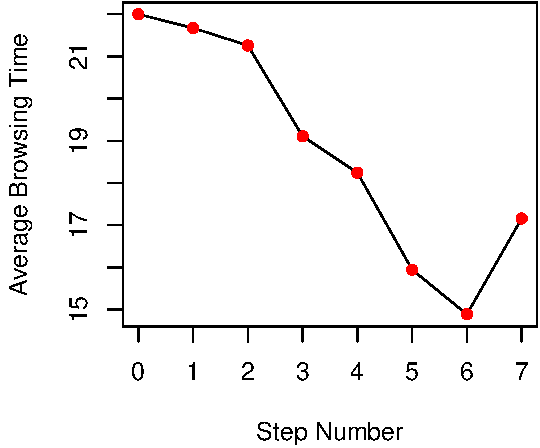
\includegraphics[width=0.5\textwidth]{nf3.pdf}
                  \caption{Average browsing time along the path of steepest descent.}\label{fig:nf3}
            \end{figure}
      \item[*] Clearly that Step 6 corresponded to the lowest observed average browsing time, and so we should
            perform another test of curvature in this region to determine whether we've reached the vicinity of the
            optimum.
      \item In order to do so, another $2^2$ factorial experiment with a centre point needs to be run. The factor
            levels in coded and natural units for this next experiment are shown in~\Cref{tab:netflixtab3}.
            \begin{table}[!htbp]
                  \centering
                  \caption{Average browsing time by condition in the second $2^2 + \symbfsfup{CP}$ Netflix experiment.}\label{tab:netflixtab3}
                  \begin{tabular}{cccccc}
                        \toprule Condition & Preview Length & $x_{1}$ & Preview Size & $x_{2}$ & Average Browsing Time \\
                        \midrule 1         & 60 seconds     & $-1$    & $0.6$        & $-1$    & $14.57$ minutes       \\
                        2                  & 90 seconds     & $+1$    & $0.6$        & $-1$    & $18.17$ minutes       \\
                        3                  & 60 seconds     & $-1$    & $0.8$        & $+1$    & $18.22$ minutes       \\
                        4                  & 90 seconds     & $+1$    & $0.8$        & $+1$    & $18.65$ minutes       \\
                        5                  & 75 seconds     & 0       & $0.7$        & 0       & $14.83$ minutes       \\
                        \bottomrule
                  \end{tabular}
            \end{table}
      \item Once again we fit a linear regression model with linear predictor:
            \[ \eta=\beta_0+\beta_1x_1+\beta_2x_2+\beta_{12}x_1x_2+\beta_{\symbfsfup{PQ}}x_{\symbfsfup{PQ}} \]
      \item The resulting output is shown below:
            \verbatiminput{verbatim/netflixOUT3.txt}
            \begin{itemize}
                  \item Reject $ \HN $: $ \beta_{\symbfsfup{PQ}}=0 $, therefore we conclude there is a quadratic curve.
            \end{itemize}
\end{itemize}
